\section{SLAM}

Simultaneous Localization And Mapping (SLAM)\cite{FirstSLAMMention}\cite{SLAMIntro} refers to both the problem and the algorithms that tries to solve it. The problem is to incrementally build a map of landmark observations, while also locating the agent which observes these measurements in the map. Popular solutions to this include EKF-SLAM\cite{EKFSLAM}, FastSLAM\cite{FastSLAM1} and factor graph\cite{Dellaert} solutions like iSAM2\cite{iSAM2}. These solutions are explained in detail below. 

The problem is usually formulated probabilistic. The important variables used in the formulation are the following:

\begin{itemize}
    \item $x_k$: The pose of the agent at time $k$. 
    \item $u_k$: The vector of inputs that move the agent to the pose $x_k$ at time $k$.
    \item $m_i$: A vector containg the location of the $i$th landmark in the map frame. 
    \item $z_k$: A vector of all the measurements of the relative positions of landmarks that can be measured from the agent at time $k$ 
\end{itemize}

There is also a number of sets that are needed

\begin{itemize}
    \item $X_{0:k} = \{x_0,x_1,...x_k\} = \{X_{0:k-1},x_k\}$: The history of all the agents poses.
    \item $U_{1:k} = \{u_1,u_2,...,u_k\} = \{U_{1:k-1},u_k\}$: The history of all control inputs.
    \item $m=\{m_1,m_2,...,m_n\}$: The set of all landmarks, also called the map.
    \item $Z_{0:k}=\{z_0,z_2,...,z_k\} = \{Z_{0:k-1},z_k\}$: The set of all landmark observations that have been measured until time $k$.
\end{itemize}

The problem can now be formulated as computing the probability distribution 

\begin{equation}
    P(x_k,m|Z_{0:k},U_{0:k},x_0)
\end{equation}

at every time step $k$. This is the joint posterior density of the location of all landmarks in the map and the agents pose, given all the measurements that have been seen so far and the control inputs that have been applied to the agent, as well as the initial pose. 

One usually wants to compute this distribution reccursively. This is done by using the previously computed distribution $P(x_{k-1},m|Z_{0:k-1},U_{0,k-1},x_0)$ at the previous time step $k-1$, together with a model for the next pose of the agent given the current input and pose, 

\begin{equation}
    P(x_k|x_{k-1},u_k)
\end{equation}

and a measurement model, giving the probability of making an observation $z_k$ of landmarks, when both the agents pose and the landmark locations are known

\begin{equation}
    P(z_k|x_k,m)
\end{equation}

The standard way of doing it now is doing a two part update of to get the desired distribution. First a time update, that uses the motion model to find an estimate for the agents location


\begin{align}
    P(x_k,m|Z_{0:k},U_{0:k}, x_0) 
     = & \int P(x_k|x_{k-1},u_k) \\
    & \times P(k_{k-1},m|Z_{0:k-1},U_{0:k-1},x_0)dx_{k-1}
\end{align}

The second update is to include the effect of measurements, 

\begin{equation}
\begin{split}
    P(x_k,m|Z_{0:k},U_{0:k},x_0) 
    = \frac{P(z_k|x_k,m)P(x_k,m|Z_{0:k-1},U_{0:k},x_0)}{P(z_k|Z_{0:k-1},U_{0:k}}
\end{split}
\end{equation}

How the method describes the motion model and measurement model, and how it does the two updates differ from method to method, but this is the main idea that lies behind them all. The SLAM problem has been said to have been solved, but this is only meant theoretically; in practice there are still problems with all of the methods. The main challenges that are still not overcome completely are 

\begin{itemize}
    \item How to update in real time.
    \item How to build a consistent map that doesn't make the computational demand grow exponentially.
    \item How to associate measurements to landmarks.
\end{itemize}

\subsection{EKF}

One of the first solution to the SLAM problem was the EKF-SLAM\cite{EKFSLAM}. It assumes a motion model 

\begin{equation}
    P(x_k|x_{k-1},u_k) \iff  x_k = f(x_{k-1},u_k) + w_k
\end{equation}

where $f(x_{k-1},u_k)$ is the model of the vehicle kinematics and $w_k$ is additive, zero mean, uncorrelated Gaussian noice with covariance $Q_k$. The observation model is similarily assumed to be 

\begin{equation}
    P(z_k|x_{k-1},m) \iff  z(k) = h(x_{k},m) + v_k
\end{equation}

where $h$ is a function describing the geometry of the observations and $v_k$ is additive, zero mean, uncorrelated Gaussian noise with covariance $R_k$. 

Using the above models, the standard EKF can be used to compute the mean 

\begin{equation}
    \begin{bmatrix} \hat{x}_{k|k} \\ \hat{m}_k \end{bmatrix} = E[\begin{bmatrix} x_k \\ m \end{bmatrix} | Z_{0:k}]
\end{equation}

and the covariance

\begin{align}
    P_{k|k} &= \begin{bmatrix} P_{xx} & P_{xm} \\ P^T_{xm} & P_{mm} \end{bmatrix} \\
     &= E\bigg[\begin{bmatrix} x_k-\hat{x}_k \\ m - \hat{m}_k\end{bmatrix}\begin{bmatrix} x_k-\hat{x}_k \\ m - \hat{m}_k\end{bmatrix}^T \bigg| Z_{0:k} \bigg]
\end{align}

of the desired joint posterior distribution $P(x_k,m|Z_{0:k},U_{0:k},x_0)$. This is done by first time-updating using

\begin{align}
    \hat{x}_{k|k-1} &= f(\hat{x}_{k-1|k-1},u_k)
    P_{xx,k|k-1} &= \nabla f P_{xx,k-1|k-1}\nabla f^T + Q_k 
\end{align}

Here $\nabla f$ is the jacobian of f at the previous estimate $\hat{x}_{k-1|k-1}$. The landmarks aren't updated, since they are assumed stationary. The measurement update is then

\begin{align}
    \begin{bmatrix} \hat{x}_{k|k} \\ \hat{m}_k \end{bmatrix} &= 
    \begin{bmatrix} \hat{x}_{k|k-1} \\ \hat{m}_{k-1} \end{bmatrix}
    + K_k[z(k) - h(\hat{x}_{k|k-1},\hat{m}_{k-1})] \\
    P_{k|k} &= P_{k|k-1} - K_kS_kK_k^T
\end{align}

where the innovation, $S_k$, is defined as

\begin{equation}
    S_k = \nabla hP_{k|k-1}\nabla h^T + R_k
\end{equation}

and the Kalman gain, $K_k$, is defined as

\begin{equation}
    K_k = P_{k|k-1}\nabla h^T S_k^{-1}
\end{equation}

Here $\nabla h$ is the jacobian of h computed at $\hat{x}_{k|k-1}$ and $\hat{m}_{k-1}$. 

This solution to the SLAM problem has been proven to converge if the motion model and measurement model is correct. It does however suffer from a quadratically growing complexity in the number of landmarks, and will not be possible to implement in real time if the total map size gets too big. It also is very sensitive to incorrect associations between measurements and landmarks and since it is a linear approximation to the true model, it has the same problems that the EKF does in terms of divergence from the true solution. 

\subsection{FastSLAM}

Theoretically, one could use a particle filter\cite{ParticleFilter} to solve the SLAM problem. But practically, the particle filter can't deal with the high dimensionality of the state space, making it computationally unfeasible without any modifications. One such modification is the Rao-Blackwellized Particle Filter (RBPF)\cite{RBPF}. It assumes it's possible to partition the state, $\xi$, into two states, $\xi_1$ and $\xi_2$, that has a joint probability distribution 

\begin{equation}
    P(\xi_1,\xi_2) = P(\xi_2|\xi_1)P(\xi_1)
\end{equation}

where the conditional probability $P(\xi_2|\xi_1)$ is possible to represent analytically. This means that only $P(\xi_1)$ needs to be represented by sampling particles. The effect of this is that the marginal $P(\xi_2)$ is possible to compute with less particles, greatly reducing the computational complexity. 

Applying this mindset to the SLAM problem results in what is known as FastSLAM\cite{FastSLAM1}. The idea is that since the error in landmarks will all depend on the error in pose, the pose is the only variable in $\xi_1$. The remaining set of variables, $\xi_2$, is then the map, which is found by conditioning on the state and the measurements. This leads to the following factorization of the joint distribution

\begin{equation}
    P(X_{0:k},m|Z_{0:k},U_{0:k},x_0) = P(m|X_{0:k},Z_{0:k})P(X_{0:k}|Z_{0:k},x_0)
\end{equation}

Furthermore, it is assumed that the landmarks are independent of each other, i.e. that the joint landmark distribution $P(m|Z_{0:k},x_0)$ can be written as the product of each landmarks distribution

\begin{equation}
    P(m|X_{0:k},Z_{0:k}) = \prod_{1<i<n}P(m_i|X_{0:k},Z_{0:k})
\end{equation}

The method then employs $R$ particles, that each represent a pose, calculated by using a normal particle filter by propagation using a motion model, weighting using the measurement model and resampling. Each particle has a map, that is calculated analytically by the particle trajectory, measurements and the measurement model. This is the same as saying that each particle has a set of $n$ small EKFs, that each try to estimate the position of each landmark. 

The independence assumption between the landmark distributions mean that the complexity of the computations can be kept to $Rlog(n)$, compared to $n^2$ of the EKF-SLAM. 

There are two different version of FastSLAM: FastSLAM 1.0\cite{FastSLAM1} and FastSLAM 2.0\cite{FastSLAM2}. The difference lies in the proposal and weighting functions. 

FastSLAM 1.0 uses the motion model 

\begin{equation}
    x_{k,i} ~ P(x_k|x_{k-1,i},u_k)
\end{equation}

as a proposal function, which gives that the weights are calculated using the marginalized observation model

\begin{equation}
    w_{k,i} = w_{k-1,i}P(z_k|X_{0:k,i},Z_{0:k-1})
\end{equation}

For FastSLAM 2.0 however, the proposal function uses the latest observation $z_k$,

\begin{align}
    x_{k,i} &= P(x_k|X_{0:k-1,i},Z_{0:k},u_k) \\
    &= \frac{1}{C}P(z_k|x_k,X_{0:k-1,i},Z_{0:k})P(x_k|x_{k-1,i},u_k)
\end{align}

Where C is a normalizing constant. This gives that the importance weights are calculated as

\begin{equation}
    w_{k,i} = w_{k-1,i}C
\end{equation}

According to \cite{SLAMIntro} this leads to a weighting function that is locally optimal. This means that it gives the smallest posible variance in the weight $w_{k,i}$, given $X_{0:k-1,i}$, $Z_{0:k}$ and $U_{0:k}$.

\subsection{Factor graph based approaches}

One new developement in the SLAM community is the developement of factor graph based approaches. This is by many considered state of the art, and some of the algorithms to come out of this approach tackles issues that haven't been possible to solve other ways. In the following the factor graph and some of the algorithms that use it are explained. The subject is graphical in nature, and a few examples are therefore in place. Many of the main points of the discussion are paraphrased from Frank Dellaert's amazing book on the subject\cite{Dellaert}.

\subsubsection{Bayesian network}

One very intuitive way of representing the SLAM problem is through a Bayesian network, or Bayes net for short. It's a graphical way of representing a joint probability density function that easily shows the different conditionings and relationships between variables. 

To be more precise, a Bayes net tries to model the joint pdf, $p(\theta)$, of all the random variables of interest, $\Theta = \{\theta_1, ..., \theta_n\}$, as a product of conditional probabilities

\begin{equation}
    p(\Theta) = \prod_j p(\theta_j|\pi_j)
\end{equation}

where $\pi_j$ is the set of variables that $\theta_j$ depends on. For the offline SLAM problem the variables of interest would be the set of poses, $X$, and the set of measurements, $Z$, that the agent has been in and observed, respectively, as well as the location of all the landmarks, also known as the map $m$. In other words, $\Theta = \{X,Z,m\}$. 

This is best illustrated through an example. Let's say we have a two poses, $x_1$ and $x_2$. The first pose we have an initial guess on, $p(x_1)$, and $x_1$ is also measured. Call this measurement $z_1$, with measurement model $p(z_1|x_1)$. In addition we have a conditional probability distribution on the second pose given the first, $p(x_2|x_1)$. This is called the motion model. 

There are two landmarks, $m_1$ and $m_2$, with pdfs on their location $p(m_1)$ and $p(m_2)$. In the first pose the agent measured the location of $m_1$ relative to himself. Call this measurement $z_2$. It has a measurement model that depends on both the landmark and the pose of the agent, $p(z_2|x_1,m_1)$. Similarily the agent also measured $m_2$ from pose $x_1$ and from pose $x_1$. Call these measurements $z_3$ and $z_4$ respectively, with corresponding measurement models, $p(z_3|x_1,m_2)$ and $p(z_4|x_2,m_2)$. 

\begin{figure}
    \centering
    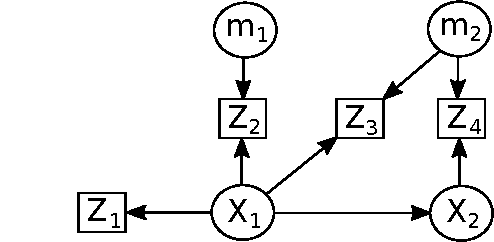
\includegraphics[width=0.8\linewidth]{0_Images/3_Background/BayesNet.pdf}
    \caption[Example of a Bayes net.]
    {Example of a Bayes net, used for a simple SLAM problem. The $x_i$'s represent poses, $z_i$'s represent measurements and $m_i$'s represent landmarks.}
    \label{Fig:BayesNet}
\end{figure}

This is represented as a Bayes net in figure \ref{Fig:BayesNet}. Here the arrows imply that the variable being pointed to depends on the variable the arrow points away from. This way all the conditional probabilities are easy to see. The Bayes net leads to the following factorization of the joint distribution

\begin{align}
    p(\Theta) = \; & p(x_1)p(x_2|x_1) \\
    \times \; &p(m_1)p(m_2) \nonumber \\
    \times \; &p(z_1|x_1) \nonumber \\
    \times \; &p(z_2|x_1,m_1) \nonumber \\ 
    \times \; &p(z_3|x_1,m_2)p(z_4|x_2,m_2) \nonumber 
\end{align}

In a SLAM setting one usually don't have any priors on the map or the initial pose, so $p(x_1)$, $p(m_1)$ and $p(m_2)$ are dropped. 

How these pdf's look depends on sensor setup and application. The model for a measurement $z_i$ is often assumed to be of the type

\begin{equation}
    z_i = h(x_k,m_i) + v
\end{equation}

where $h(x,m_i)$ is the measurement function of the landmark $m_i$ at the pose $x_k$, and $v$ is zero-mean white noise with the so-called measurement covariance $R$. This means the pdf of $z_i$ given $x_k$ and $m_i$ is 

\begin{equation}
    p(z_i|x_k,m_i) = \frac{1}{\sqrt{2\pi R}}exp(-1/2||h(x_k,m_i) - z_i||^2_R)
\end{equation}

The measurement function depends on the sensor used and how the poses and landmarks are represented. For a bearing measurement in the plane, with landmarks being two-dimensional vectors and the pose represented as a point in the plane and a heading, the measurement function could be represented as

\begin{equation}
    h(x_k,m_i) = atan2(m_{i,y} - x_{k,y},m_{i,x} - x_{k,x})
\end{equation}

Similarily for the pdf of the pose step, it is often modeled as a gaussian, but now using the motion model, $g(x_k,u_k)$ instead of the measurement function. 

\begin{equation}
    p(z_i|x_k,m_i) = \frac{1}{\sqrt{2\pi R}}exp(-1/2||g(x_k,u_k) - z_i||^2_R)
\end{equation}

In Revolve's case the input can be thought of as the estimated body linear and angular velocities $v_{x,k}$, $v_{y,k}$ and $r_k$ at step $k$. Then the motion model becomes 

\begin{equation}
    \begin{bmatrix} x_k \\ y_k \\ \psi_k \end{bmatrix} = \begin{bmatrix} x_{k-1} \\ y_{k-1} \\ \psi_{k-1} \end{bmatrix} + \begin{bmatrix} cos(\psi_{k-1})v_{x,k} - sin(\psi_{k-1})v_{y,k} \\
    sin(\psi_{k-1})v_{x,k} + cos(\psi_{k-1})v_{y,k} \\ r
    \end{bmatrix} dt
\end{equation}

where $dt$ is the time increment.

\subsubsection{MAP}

The Bayes net has given us a way of setting up the joint probability density function for both the pose, landmarks and measurements. In SLAM we are typically interested not in this joint pdf, but in the set of poses and landmark locations that maximizes the joint pdf, given the measurements. The usual way of estimating these values is to use the maximum a posteriori (MAP) estimate. In offline SLAM this equates to finding the estimated path, $X$, and map, $m$, that maximizes the conditional density $p(X,m|Z)$. In symbols

\begin{align}
    (X,m)^{MAP} &= \argmax_{X,m}p(X,m|Z) \\
    &= \argmax_{X,m}\frac{p(Z|X,m)p(X,m)}{p(Z)}
\end{align}

The second equality is simply using Bayes rule. Since the measurements are given, we drop the normalization constant $p(Z)$. This gives

\begin{equation}
    (X,m)^{MAP} = \argmax_{X,m}l(Z|X,m)p(X,m)
\end{equation}

where the first term, $l(Z|X,m)$ is no longer a proper pdf, but now just a likelihood function proportional to $p(Z|X,m)$. Note that in general, conditioning on the measurements means the likelihood function does not look like a gaussian.

Even though the Bayes net gives a nice way of representing the problem that is easily understandable, it offers no good way of doing inference, like finding the MAP estimate. This is the reason why factor graphs have been developed, as the way they are built lends room for optimizations like this.

\subsubsection{Factor graphs}

A factor graph is a special type of bipartite graph. A bipartite graph is a graph that can be divided into two disjoint and independent sets, where each node in one set has edges to nodes in the other set, but not any edges connecting them to nodes in the same set. The two sets of nodes in a factor graph are factors $\phi_i\in \mathcal{U}$ and variables $x_j\in \mathcal{V}$. Since it is bipartite, edges $e_{ij}\in \mathcal{E}$ are therefore only between factors and variables. 

The set of all the variables that have edges to a certain factor $\phi_i$ is written as $\Theta_i$, which is a subset of the set of all the variables $\Theta = \{X,m\}$. The factor graph now represent a factorization of a function $\phi(\Theta)$ as the product of all the factors, where each factor is a function of only the variables that have edges to it.

\begin{equation}
    \phi(\Theta) = \prod_i \phi_i(\Theta_i)
\end{equation}

A Bayes net can be converted to a factor graph through a simple transformation. Every node in the net that is not given is split into two; a variable and a factor. The given variables are simply omitted, and become fixed parameters in the factors. 

This means that in the example in figure \ref{Fig:BayesNet}, since the measurements are given, they are absorbed into the nodes adjacent to them. The rest of the nodes, i.e. the poses and the landmarks are split into variables and factors. Variables that used to be connected via a measurement are now connected to the same factor. The corresponding factor graph of the above example is shown in figure \ref{Fig:FactorGraph}. Here a dot indicates a factor. There are factors for each of the landmark measurements and for the measured initial pose as well as the relative pose between $x_1$ and $x_2$. There are also factors for the prior on the initial pose and priors on the landmarks.

\begin{figure}
    \centering
    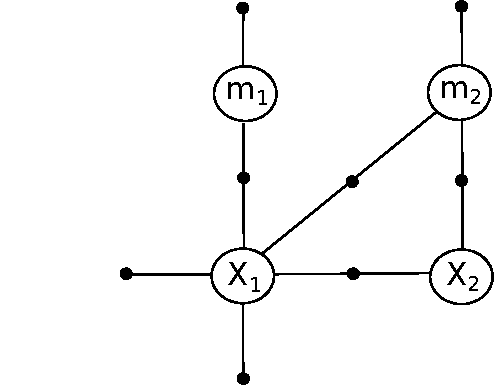
\includegraphics[width=0.8\linewidth]{0_Images/3_Background/FactorGraph.pdf}
    \caption[Example of a Bayes net.]
    {Example of a factor graph, obtained by converting the Bayes net example in figure\ref{Fig:BayesNet} into a factor graph.}
    \label{Fig:FactorGraph}
\end{figure}

\subsubsection{Inference on factor graphs}

The great thing about the factor graph representation is that now the MAP estimate of all the variables $\Theta$ in the factor graph is simply

\begin{align}
    \Theta^{MAP} &= \argmax_{\Theta} \phi(\Theta) \\
    &= \argmax_{\Theta}\prod_i \phi_i(\Theta_i)
\end{align}

In the case of likelihood factors derived from measurements corrupted by zero-mean, normally distributed noise, as discussed above, the factors are proportional to

\begin{equation}
    \phi_i(\Theta_i) \propto exp(-\frac{1}{2}||h_i(\Theta_i) - z_i||_{\Sigma_i}^2)
\end{equation}

To avoid numerical errors stemming from adding numbers of very different order of magnitude, we take the negative log of this and drop the factor of $1/2$. This gives us the following minimization objective

\begin{equation}
    \Theta^{MAP} = \argmin_{\Theta}\sum_i ||h_i(\Theta_i) - z_i||_{\Sigma_i}^2
\end{equation}

This amounts to a nonlinear least-squares. This problem can be solved by nonlinear optimization methods such as Steepest Descent, Gauss-Newton, Levenberg-Marquardt or Dogleg minimization, and will converge to a global minima if given a good initial guess. Nocedal and Wright\cite{NumOpt} has an excellent book on the subject if more information is needed. Most of the optimization methods linearize the cost function and use this to find a step that takes them closer to the minimum, but as long as the factors are analytically expressed the whole cost function $\phi(\Theta)$ is possible to evaluate. This means that methods based on random sampling, like Markov Chain Monte Carlo and Gibbs sampling\cite{SamplingOpt} might also be suitable. The following discussion will however focus on gradient-based method using linearization.

Linearizing the above cost-function around the current estimate $\Theta^0$, leads to a linear least-squares problem giving the optimal step in state $\Delta*$

\begin{align}
    \Delta* &= \argmin_{\Delta}\sum_i ||h_i(\Theta_i^0) + H_i\Delta_i - z_i||_{\Sigma_i}^2 \\ 
    &= \argmin_{\Delta}\sum_i || H_i\Delta_i - (z_i - h_i(\Theta_i^0))||_{\Sigma_i}^2
\end{align}

where $z_i - h_i(\Theta_i^0)$ is the error between the actual and predicted measurement given the estimate of the relevant variables. By a change of basis, scaling the different variables such that the optimization becomes a sum of euclidian norms, this can again be rewritten as 

\begin{align}
    \Delta* &= \argmin_{\Delta}\sum_i||A_i\Delta_i - b_i||_2^2 \\
    &= \argmin_{\Delta}||A\Delta - b||_2^2
\end{align}

This equates to solving the following for the optimal step $\Delta*$

\begin{equation}
    (A^TA)\Delta* = A^Tb
\end{equation}

This can be done through QR or Cholesky factorization. Both these algorithms amount to finding a factorization of the system that makes it easy to solve. In Cholesky factorization this is done by factorizing it as $A^TA = R^TR$, where $R$ is an upper triangular $n \times n$ matrix. When you have this factorization, solving the system is just solving 

\begin{equation}
    R^Ty = A^Tb
\end{equation}

by forward substitution, then 

\begin{equation}
    R\Delta* = y
\end{equation}

by back-substitution. 

QR-factorization is a more numerically stable and accurate method that achieves the same goal by instead finding a factorization of $A$ 

\begin{equation}
    A = Q\begin{bmatrix} R \\ 0 \end{bmatrix}
\end{equation}

and a corresponding right hand side

\begin{equation}
    \begin{bmatrix} d \\ e \end{bmatrix} = Q^Tb
\end{equation}

Solving 

\begin{equation}
    R\Delta* = d
\end{equation}

by back-substitution then gives the desired step $\Delta*$.

\subsubsection{Sparsity}

In SLAM the matrix A, and the resulting information matrix $A^TA$ are usually really sparse, because of the following three properties

\begin{itemize}
    \item The poses are linked linearily.
    \item No factors between landmarks.
    \item Relatively few factors from each landmark.
\end{itemize}

These properties together means that each factor in the graph depends on only a small set of variables, which amounts to sparsity of $A$ and $A^TA$. This sparsity can be used to speed up the optimization, using sparse factorization schemes like sparse Cholesky or LDL factorization\cite{SparseLinearAlgebra}. 

\subsubsection{Incremental inference}

Throughout the above discussion the factor graph was applied to the problem of offline or batch SLAM, where the desired objective is to find the set of poses and landmarks that is most probable, given all the measurements. This is however not the same setting as Revolve NTNU is faced with, which is incremental SLAM.

In incremental SLAM the map is built up gradually, and care must be taken so the computation time does not keep increasing as the number of landmarks increase. In formula student the map is finite, as the track eventually loops, but even so there are strict constraints on how much computation time the optimization can afford. To drive fast the time from detection to map and correction on pose must be minimized. A delay might mean the car hits a delimiter that it could have known about.

The problem is thus one of incremental inference, and can be seen as successively solving batch SLAM problems, where at each step the new problem is just the previous problem with some added constraints from the new measurements.

For the nonlinear least-squares problem that comes from adding gaussian zero-mean noise to the measurement and motion models, this problem can tackled by reusing as much as possible of the previous QR-factorization. Naively one might update, relinearize and refactorize the entire cost function using QR-factorization every time new measurements arrive. Instead one could use a process called QR-updating to add the new information directly to the QR-factorized linearized system. 

In QR-updating measurements are just thought of as adding a new row $a^T$ to previous factor R and a new scalar element $\beta$ to the right hand side $d$. This yields a new system $R_d|d_a$ that is not in the correctly factorized form

\begin{equation}
    R' = \begin{bmatrix} R \\ a^T \end{bmatrix}=\begin{bmatrix} Q^T &  \\ & a \end{bmatrix}\begin{bmatrix} A \\ a^T \end{bmatrix} \quad \quad d_a' = \begin{bmatrix} d \\ \beta  \end{bmatrix}
\end{equation}

This is then moved into the right form by successive applications of Givens rotations\cite{GivensRot}. Without going into too much detail, the Givens rotations succesively remove one and one element from the bottom row, possibly adding terms higher up, which are then also removed later. After a certain amount of rotations the matrix $R'$ is in upper triangular form, which means the linear least square is easy to solve.

\subsubsection{Bayes tree}

The above solution allows incremental updating of the linearized system. Its memory usage and computation time are however still unbounded over time. It also will tend to fill in the previously sparse information matrix as the algorithms keep iterating, thus making the back substitution more and more demanding.

The problem of increased memory usage and computation time is in part solved in iSAM2 via marginalization over time. This means removing variables from the optimization without removing the information they encode. This corresponds to integrating out the variable we want eliminated, $y$, from the joint pdf of $y$ and the rest of the variables $X$, yielding a new pdf that is only over the remaining variables

\begin{equation}
    p(X) = \int_yp(X,y)dy
\end{equation}

For a gaussian density represented as 

\begin{equation}
    p(x,y) = \mathcal{N}(\begin{bmatrix}\mu_x \\ \mu_y \end{bmatrix}, \begin{bmatrix} \Sigma_{xx} & \Sigma_{xy} \\ \Sigma_{xy}^T & \Sigma_{yy} \end{bmatrix}) 
\end{equation}

this is nothing more than just picking the relevant mean and covariance to get the new pdf

\begin{equation}
    p(y) = \mathcal{N}(\mu_x,\Sigma_{yy})
\end{equation}

To achieve marginalization of a factor graph however, and to avoid that the Givens rotations needed for incremental updating of the factorization eventually makes the information matrix dense, more sophisticated tools are required. The tools that iSAM2 uses are bipartite eliminitation\cite{BipartElim} and the Bayes tree\cite{BayesTree}. 

Bipartite elimination refers to converting a factor graph into a chordal Bayes net by eliminating one and one variable from the factor graph until only the bayes net remains. Elimination of a variable $\theta_j$ implies the following steps (replicated from \cite{iSAM2} for completeness)

\begin{itemize}
    \item Remove from the factor graph all factors $\phi_i(\Theta_i)$ that are adjacent to $\theta_j$. Define the separator $S_j$ as all variables involved in those factors excluding $\theta_j$.
    \item Form the (unnormalized) joint density $f_{joint}(\theta_j,S_j) = \prod_i\phi_i(\Theta_i)$ as the product of the factors in $S_j$.
    \item Usin the chain rule, factorize the joint density $f_{joint}(\theta_j, S_j) = P(\theta_j| S_j)f_{new}(S_j)$. Add the conditional $P(\theta_j|S_j)$ into the Bayes net and the factor $f_{new}(S_j)$ back into the factor graph.
\end{itemize}

The process repeats until the factor graph is completely converted into a Bayes nes.

This chordal Bayes net is then possible to transform into a Bayes tree. The Bayes tree is a directed acyclical graph built by forming cliques in the chordal Bayes tree. This is always possible, although a proof of this is not going to be presented here. The algorithm can be seen in the iSAM2 paper\cite{iSAM2}. This structure encodes the joint density of the factor graph in such a way that incremental inference is made easy and that intuitively shows the structure of the information matrix, making it easy to avoid that this gets dense over time.

Once the bayes tree is formed, adding new factors is just 

\begin{itemize}
    \item Removing the cliques which have edges to the factor, storing the orphaned sub-trees for later, and re-interpret the removed cliques as a factor graph.
    \item Add the new factors into this small factor graph.
    \item Re-order the variables of the factor graph.
    \item Eliminate into a new Bayes tree.
    \item Insert the previously orphaned sub-trees back into the new Bayes tree.
\end{itemize}

This is the gist of the iSAM2 algorithm. In addition it uses a constrained COLAMD (CCOLAMD) ordering when it reorders the variables after creating a new factor graph. The constraint are that it wants to have the newest variables at the top of the Bayes tree since they are the most likely to be affected in the next step. This constraint ensures the size of the affected part of the tree is smaller in futures steps, and COLAMD ensures overall good ordering. 

It also relinearizes only parts of the cost function. It does this by relinearizing only the variables that have gone above a threshold away from their linearization value. This is crucial for this incremental algorithm, since if batch relinearizations were needed it would make the computational cost unbounded over time. Finally, for the same reason, it updates the solution of the variables by going backwards in the Bayes tree. When the change in a variable goes below a threshold it stops updating the solutions. 